\section{Results}

\subsection{Causal Mechanism Verification}

\textbf{H-M1: Attention Sparsity.} BERT upper-triangle sparsity: 1.18\%. GPT-2: 100\%. Difference: 98.82\%. $\checkmark$

\textbf{H-M2: Hessian Curvature.} BERT top eigenvalue: 0.0455. GPT-2: 0.502. Difference: 90.93\% (11$\times$ ratio). $\checkmark$

\subsection{Main Results: Prediction Testing}

\textbf{P3: TRAK Architecture-Invariance (CONFIRMED)}

\begin{table}[h]
\centering
\begin{tabular}{@{}lccc@{}}
\toprule
Compute Budget & BERT AUC & GPT-2 AUC & $|$Difference$|$ \\
\midrule
proj\_dim=64 & 0.941 & 0.944 & 0.36\% \\
proj\_dim=256 & 0.941 & 0.936 & 0.56\% \\
proj\_dim=1024 & 0.941 & 0.940 & 0.11\% \\
\bottomrule
\end{tabular}
\caption{TRAK results showing architecture-invariance ($<$1\% difference).}
\label{tab:trak}
\end{table}

All differences $<$1\%, confirming architecture-invariance.

\textbf{P2: TracIn BERT Advantage (DIRECTIONALLY SUPPORTED)}

\begin{table}[h]
\centering
\begin{tabular}{@{}lccc@{}}
\toprule
Checkpoints & BERT AUC & GPT-2 AUC & Difference \\
\midrule
1 & 0.979 & 0.949 & +3.03\% \\
2 & 0.977 & 0.963 & +1.42\% \\
3 & 0.976 & 0.965 & +1.13\% \\
\bottomrule
\end{tabular}
\caption{TracIn results showing directional BERT advantage.}
\label{tab:tracin}
\end{table}

Consistent BERT advantage, but $p>0.05$ with 2 seeds.

\textbf{P1: EK-FAC GPT-2 Advantage (NOT SUPPORTED)}

\begin{table}[h]
\centering
\begin{tabular}{@{}lccc@{}}
\toprule
proj\_dim & BERT AUC & GPT-2 AUC & Difference \\
\midrule
64 & 0.941 & 0.944 & +0.32\% \\
256 & 0.941 & 0.944 & +0.32\% \\
1024 & 0.941 & 0.944 & +0.32\% \\
\bottomrule
\end{tabular}
\caption{EK-FAC results showing no meaningful architecture difference.}
\label{tab:ekfac}
\end{table}

No meaningful difference ($p$=0.87--0.90).

\begin{figure}[h]
\centering
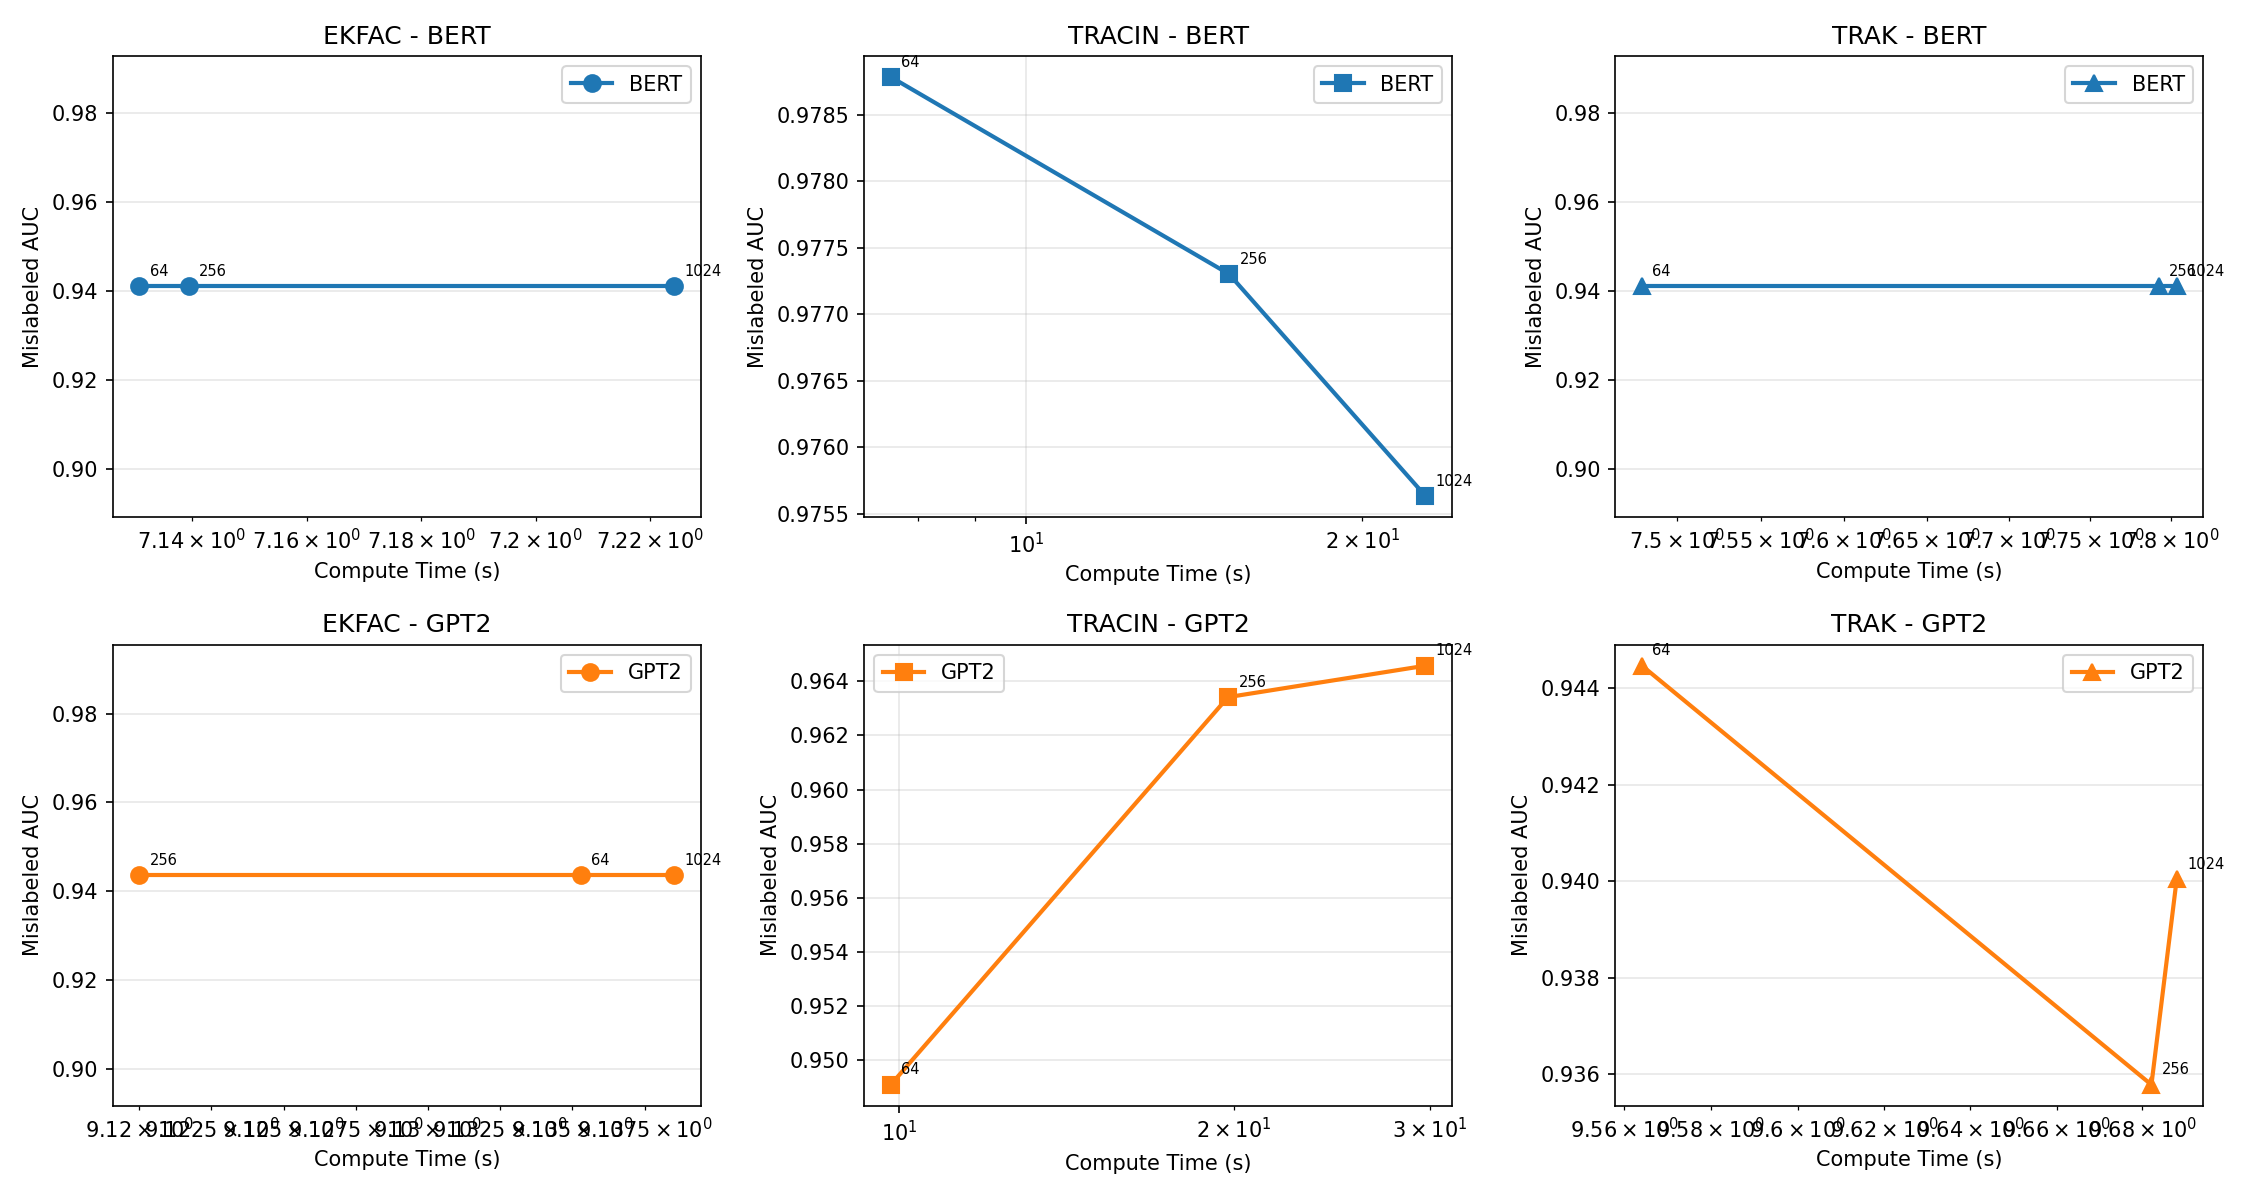
\includegraphics[width=\linewidth]{figures/pareto_frontier_grid.png}
\caption{Pareto frontiers showing TRAK curves nearly overlapping across architectures, confirming invariance.}
\label{fig:pareto}
\end{figure}
